\chapter{Results}\label{ch:results}

This chapter will provide various numerical test results of SF-PIF methods.
In order to examine the numerical capabilities of the SF method,
several well-known numerical benchmark problems are conducted,
and the traditional SSP-RK methods' results will be provided with the same initial conditions
as counterparts of SF-PIF methods for comparisons.
SF-PIF3 and SF-PIF4 will refer to the \textit{recursive} SF method in~\cref{sec:recursive_sf}
with third-order and fourth-order PIF methods, respectively,
and RK3 and RK4 will refer to the three-stage, third-order SSP-RK method~\cref{eq:ssp_rk3},
five-stage, fourth-order SSP-RK method~\cref{eq:ssp_rk4}, respectively.
The original SF approach (\cref{sec:original_sf}) with the PIF method is denoted by oSF-PIF\@.
The conventional five-point central differencing formulae~\cref{eq:pif_central_dfdx,eq:pif_central_dfdxx,eq:pif_central_dfdxy}
are used for SF-PIF and PIF methods otherwise specified.

\section{Performance of SF-PIF method}\label{sec:result_performance}
The main advantage of the PIF method is the performance gain compared to the SSP-RK methods.
This section will compare the performance of PIF methods (with or without the SF approach)
and the SSP-RK method. The main purpose of this section is to check if the SF-PIF methods provide
improved performance while maintaining the same accuracy as SSP-RK methods.
Theoretically speaking, the SF and oSF approach should not affect the solution's accuracy and stability,
so the original PIF method's results are presented for comparisons.

All test results in this section use the standard fifth-order WENO-JS method (\cref{subsec:weno})
for the spatially high-order reconstruction scheme.
Therefore, the expected truncation error is \( \mathcal{O}(\Delta s^{5}, \dt^{q}) \),
where \( q \) is the order of the temporal scheme.

\subsection{Sine wave advection}\label{subsec:sine_wave}

The first choice of the benchmark problem is the sine wave advection
to test if the desired solution accuracy is retrieved in smooth flows.
The initial condition follows the setup in~\cite{lee2017piecewise},
where the density profile is initialized with a sinusoidal wave,
\( \rho (x) = 1.5 - 0.5\sin(2\pi x)\).
The $x$-velocity and
the pressure are set as constant values of \( u = 1\) and
\( p = 1/\gamma \)
with the specific heat ratio, \( \gamma = 5/3 \).
Albeit solved using the nonlinear Euler equations, the problem is
solved in a linear regime, viz., the velocity and pressure remain
constant for all $t\ge 0$ so that the initial sinusoidal density profile
is purely advected by the constant velocity $u=1$ without any nonlinear
dynamics such as a formation of shocks and rarefactions.

\begin{figure}
    \centering
    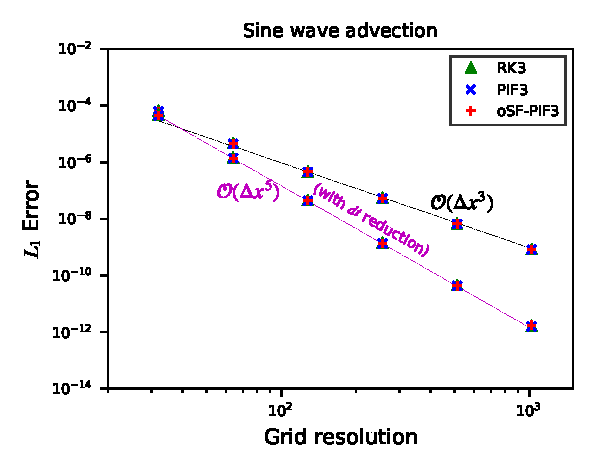
\includegraphics[width=0.85\textwidth]{fig/sine_over_dtReduction}
    \caption{Convergence test for the 1D sine wave advection problem.
        The errors are calculated
        in \( L_{1} \) sense against the initial density profile
        resolved on the computational grids refined
        from 32 to 1024 by a factor of 2.
        All numerical solutions follow the theoretical third-order convergence rate
        (the black-dotted line) when using the timesteps 
        computed from the Courant condition.
        Also plotted are the solutions of using reduced timesteps, which follows the
        fifth-order convergence rate represented in the pink-dotted line.
    }\label{fig:sine_wave}
\end{figure}

The simulation domain is defined on a one-dimensional box of \( [0, 1] \)
with the periodic boundary condition on both ends.
The density profile will propagate one period through the computational domain
and will return to its initial position at \( t = 1 \).
In return, any shape deformation of the density profile
from the initial density profile can be considered as a numerical error
associated with phase errors or numerical diffusions.
The accuracy of the numerical solutions is measured by computing \( L_{1} \) error
between the initial and the final density profiles.
The numerical experiment results from the sine wave advection test
on different number of grid points, \( N_{x} = 32, 64, 128, 256, 512, \) and \( 1024 \)
are depicted in~\cref{fig:sine_wave} for three different temporal methods, Rk3, PIF3, and oSF-PIF3.

There are two types of convergence rates demonstrated in~\cref{fig:sine_wave}.
In the first type, the numerical solutions of three different temporal methods
advanced with timesteps computed from the Courant condition with \( C_{\text{cfl}} = 0.7 \).
Interestingly, the numerical solutions from all three different temporal methods
show a third-order convergence rate, indicating that the leading error term from
third-order temporal methods dominates the spatial error from the fifth-order WENO-JS method.
These results are different from~\cref{fig:vortex_error_saturation},
calculating \( L_{1} \) error from the 2D nonlinear vortex advection case,
where the solution accuracy follows the spatial order at low-resolution regions
until the leading error of the solution is caught up by the temporal error
as computational grids get further refined to higher resolutions.
However, in this test case, the third-order temporal accuracy quickly takes control
throughout the entire range of the grid resolutions tested herein.
This solution behavior strongly supports the importance of
integrating spatially reconstructed solutions with a temporal scheme whose accuracy is
sufficiently high enough to be well comparable to that of the spatial solver.

In the second type of the convergence rate, on the other hand, the timesteps are restricted
in order to match up the lower third-order temporal accuracy with the higher fifth-order spatial accuracy.
Following the usual trick of timestep reduction in~\cite{mignone2010high},
the timestep \( \Delta t_{N} \) is manually adjusted on a grid size of \( N \)
to satisfy the equal rate of change between the spatial and temporal variations.
The restricted timestep is defined by,
\begin{equation}\label{eq:dt_reduction}
    {\Delta t_N} = {\Delta t_0} \Big( \frac{\Delta x_N}{\Delta x_0} \Big)^{\frac{5}{3}},
\end{equation}
where the sub-indices ``0'' and \( N \) refer to the time and grid scales
on a nominal coarse and fine resolution, respectively.
In the current configuration, \( \Delta x_{0} \) is the grid-scale of \( N_{x} = 32 \),
and \( \Delta t_{0} \) is the corresponding timestep subject to the Courant condition with \( C_{\text{cfl}} = 0.7 \).
With the timestep reduction, the overall leading error from the spatial and temporal methods
are matched with the fifth-order spatial accuracy of WENO5,
and the numerical solution of PIF3 and oSF-PIF3 follows the fifth-order convergence rate as expected.
In all test cases for linear advection problems, the oSF-PIF3 solutions behave
almost equally well with the solutions of the original PIF3 and RK3 both quantitatively and qualitatively.



\subsection{Nonlinear isentropic vortex advection}\label{subsec:vortex_weno}

The isentropic vortex advection problem~\cite{shu1998essentially} is one of the most popular benchmark tests
to measure the numerical method's accuracy and performance in the nonlinear case.
Although the problem is fully nonlinear, the exact solution always exists
in the form of its initial condition,
from which an isentropic vortex is advected through periodic boundaries in a 2D computational box.
The accuracy of a numerical method on a nonlinear problem
can be evaluated by comparing the final density profile with the initial condition.

The initial condition consists of a constant background mean flow with \( \rho = 1 \),
\( (u, v) = (1,1) \) and \( p =1 \) on the 2D computaional domain
with periodic boundary conditions.
The isentropic vortex is given by the velocity perturbations \( (\delta u, \delta v) \),
and the temperature perturbation \( \delta T \).
The perturbation terms are designed to set the constant entropy \( S \)
everywhere in the simulation domain, i.e., \( \delta S = 0 \).
The perturbations are given as,
\begin{equation}\label{eq:isentropic_vortex_initial}
    \left( \delta u, \delta v \right) = \frac{\epsilon}{2 \pi} e^{-\half \left( 1 - r^{2} \right)} (-y, x), \quad
    \delta T = - \frac{\left( \gamma - 1 \right) \epsilon^{2}}{8 \gamma \pi^{2}} e^{1 - r^{2}},
\end{equation}
where \( \epsilon = 5 \) is the vortex strength and \( r^{2} = x^{2} + y^{2} \).
The vortex is initially located at the domain center,
and it advects to the diagonal directions, then returns to its original position after one cycle.
The simulation domain size is doubled-up as \( [0, 20] \times [0, 20] \)
compared to the original setup in~\cite{shu1998essentially},
to prevent vortex-vortex couplings near the periodic boundaries
as reported in~\cite{spiegel2015survey}.

\begin{figure}
    \centering
    \begin{subfigure}{70mm}
        \centering
        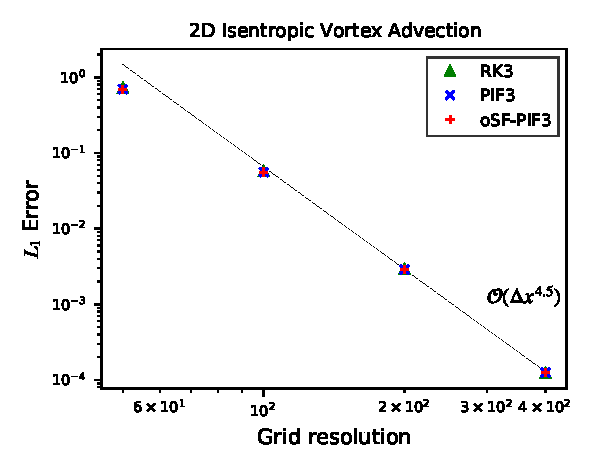
\includegraphics[width=0.95\textwidth]{fig/vortex_third}
    \end{subfigure}
    \begin{subfigure}{70mm}
        \centering
        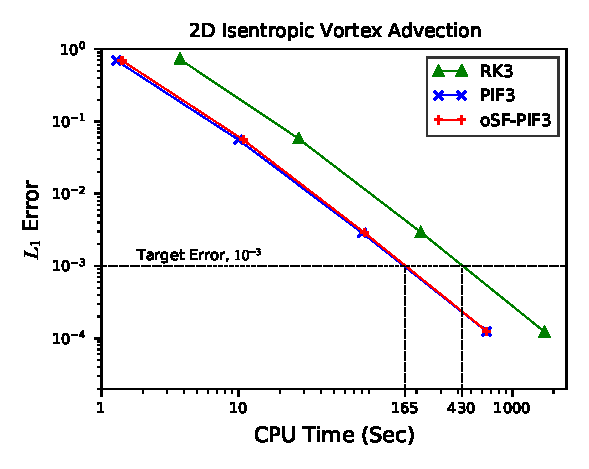
\includegraphics[width=0.95\textwidth]{fig/vortex_time_third}
    \end{subfigure}
    \caption{The \( L_{1} \) errors of the isentropic vortex advection test problem
        on different grid resolutions, \( N_{x} = N_{y} = 50, 100, 200, \) and \( 400 \).
        The three different third-order temporal schemes
        are used combined with WENO5 spatial method.
        The \( L_{1} \) errors
        with respect to the grid resolutions (\textbf{left});
        with respect to the computation time (\textbf{right}).
    }\label{fig:vortex_third}
\end{figure}

The results of the convergence test are depicted on the left panel in~\cref{fig:vortex_third}.
Three different temporal schemes, RK3, PIF3, and oSF-PIF3, show an excellent comparable match in
magnitudes and slopes of the \( L_{1} \) errors with varying grid resolution, \( N_{x} = N_{y} = 50, 100, 200, \) and \( 400 \).
One important finding in this figure is that there is no significant distinction
between PIF3 and oSF-PIF3 in accuracy and performance.
These results demonstrate that the original SF method
does not affect the solution accuracy and performance of the PIF method.

\begin{table}
    \centering
    \caption{The \( L_{1} \) errors, the rates of convergence,
        and the relative computation times for the vortex advection test.
        Here, the comparison between RK3 and oSF-PIF is only displayed,
        since the difference between oSF-PIF3 and PIF3 is indistinguishable.
        All the performance results (measured in seconds) are averaged
        over 10 simulation runs which are conducted on
        a Coffee Lake quad-core i7 Intel CPU with a
        clock speed of 2.7GHz, Turbo Boost up to 4.5GHz,
        utilizing four parallel threads.
    }\label{table:vortex_weno_third}
    \begin{adjustbox}{width=\textwidth}
        \begin{tabular}{@{}lcccclcccc@{}}
            \toprule
            \multirow{2}{*}{\( N_{x} = N_{y} \)} & \multicolumn{4}{c}{RK3} &  & \multicolumn{4}{c}{oSF-PIF3} \\
            \cmidrule(lr){2-5} \cmidrule(l){7-10}
            & \(L_{1}\) error & \(L_{1}\) order & CPU Time & Speedup &  &
            \(L_{1}\) error & \(L_{1}\) order & CPU Time & Speedup \\ \midrule
            50  & \num{7.22E-1} & \--- & \SI{3.73}{\second}    & 1.0 &  & \num{6.95E-1} & \--- & \SI{1.41}{\second} & 0.38 \\
            100 & \num{5.76E-2} & 3.65 & \SI{27.51}{\second}   & 1.0 &  & \num{5.58E-2} & 3.64 & \SI{10.82}{\second} & 0.39 \\
            200 & \num{2.94E-3} & 4.29 & \SI{214.44}{\second}  & 1.0 &  & \num{2.89E-3} & 4.27 & \SI{83.21}{\second} & 0.39 \\
            400 & \num{1.22E-4} & 4.59 & \SI{1727.71}{\second} & 1.0 &  & \num{1.26E-4} & 4.52 & \SI{652.18}{\second} & 0.38
        \end{tabular}
    \end{adjustbox}
\end{table}

The performance results of three different temporal schemes are presented
on the right panel of~\cref{fig:vortex_third} and summarized in~\cref{table:vortex_weno_third}.
Both the PIF3 and oSF-PIF3 methods perform more than two times faster than the multi-stage method, RK3.
It is worth noting that the original SF-PIF method, oSF-PIF, can be readily swappable
with an RK integrator in an existing code without too much effort,
leaving any existing spatial implementations intact.
Moreover, such a code transformation with oSF-PIF is more advantageous in simplicity
than the original PIF method because oSF-PIF replaces the analytic derivations of the Jacobian and Hessian terms
with the system-free approximations,
which have shown to be highly commensurate with
the analytical counterparts of the original PIF scheme.

Unlike the 1D linear sine advection test in~\cref{subsec:sine_wave},
the overall solution accuracy is not completely dominated by the third-order temporal discretizations,
which could reduce the overall convergence rate down to third-order as observed in the sine advection case.
Concurrently, the solution does not converge at full fifth-order either,
the rate due to the use of WENO5.
This can be explained as a nonlinear effect in which the lower third-order time integration schemes
slightly compromise the overall leading error term of the fifth-order spatial discretization.

\begin{figure}
    \centering
    \begin{subfigure}{70mm}
        \centering
        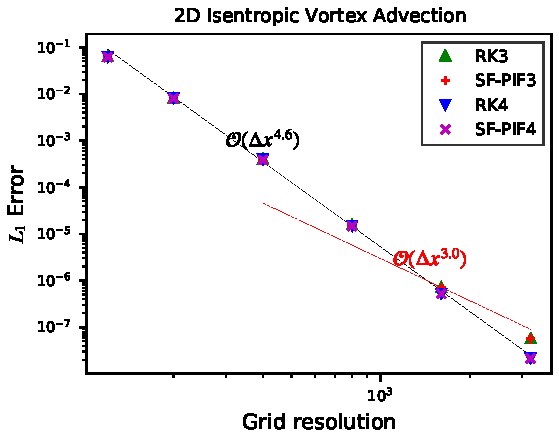
\includegraphics[width=0.95\textwidth]{fig/weno5_vortex_error_fourth}
    \end{subfigure}
    \begin{subfigure}{70mm}
        \centering
        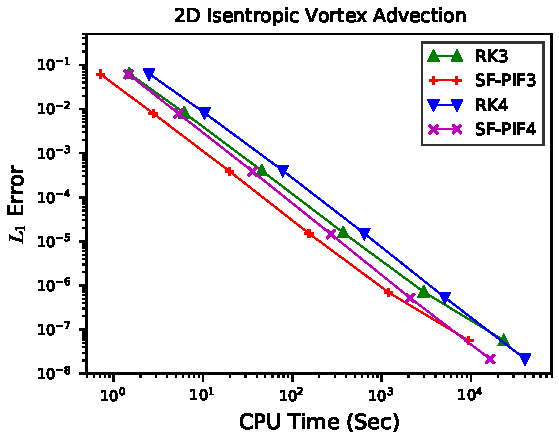
\includegraphics[width=0.95\textwidth]{fig/weno5_vortex_time_fourth}
    \end{subfigure}
    \caption{The \( L_{1} \) errors of the isentropic vortex advection test problem
        solved by third- and fourth-order temporal schemes combined with WENO5 spatial method.
        The \( L_{1} \) errors
        with respect to the grid resolutions (\textbf{left});
        with respect to the computation time (\textbf{right}).
    }\label{fig:vortex_fourth}
\end{figure}

However, the third-order temporal schemes gradually degrade the overall solution accuracy
on the fine grid resolutions. \cref{fig:vortex_fourth} illustrates the same convergence test results,
but in this case, containing more higher grid resolutions, \( N_{x} = N_{y} = 120, 200, 400, 800, 1600, \) and \( 3200 \).
Notice that the recursive SF-PIF method, SF-PIF3, and SF-PIF4 are used instead of the original SF-PIF method.
As expected, all temporal methods follow the convergence line of order \( \sim \mathcal{O}(\dx^{4.5}) \),
which is nearly the same as WENO's fifth-order spatial accuracy, equivalently in~\cref{fig:vortex_third}.
However, at the critical grid resolution, \( N_{x} = N_{y} = 1600 \),
the third-order temporal schemes of RK3 and SF-PIF3 start to compromise the overall solution accuracy.
This behavior can be explained that the spatial errors from the fifth-order WENO method
are dominant on the grid resolutions up to \( N_{x} = N_{y} = 1600 \),
after which the truncation errors associated with the third-order temporal methods
become dominant over the error of the fifth-order spatial solver, WENO5.
This result emphasizes the importance of high-order temporal methods in fine grid resolution:
a high-order spatial method does require a \textit{comparably} high-order temporal method
to maintain the overall quality of the solutions,
mainly when adding more grid resolutions to resolve finer scales more accurately.
Otherwise, lower-order accuracy from the temporal solver can potentially degrade
the solution accuracy, contradicting the intended motivation.

\begin{table}
    \centering
    \caption{The \( L_{1} \) errors, the rates of convergence,
        and the computation times for the vortex advection test
        solved using RK3 and SF-PIF3 methods (\textbf{top});
        using RK4 and SF-PIF4 methods (\textbf{bottom}).
        All simulation runs are performed on the four 20-cores
        Cascade Lake Intel Xeon processors, utilized 64 parallel threads.
        CPU times are measured in seconds, averaged over 10 individual runs.
    }\label{table:vortex_weno_fourth}
    \begin{adjustbox}{width=\textwidth}
        \begin{tabular}{@{}ccccclcccc@{}}
            \toprule
            \multirow{2}{*}{\( N_{x} = N_{y} \)} & \multicolumn{4}{c}{RK3} &  & \multicolumn{4}{c}{SF-PIF3} \\
            \cmidrule(lr){2-5} \cmidrule(l){7-10}
            & \(L_{1}\) error & \(L_{1}\) order & CPU Time & Speedup &  &
            \(L_{1}\) error & \(L_{1}\) order & CPU Time & Speedup \\ \midrule
            120  & \num{6.31E-2} & \--- & \SI{1.50}{\second}      & 1.0 &  & \num{6.16E-2} & \--- & \SI{0.71}{\second}    & 0.48 \\
            200  & \num{8.20E-3} & 4.00 & \SI{6.17}{\second}      & 1.0 &  & \num{7.96E-3} & 4.00 & \SI{2.77}{\second}    & 0.45 \\
            400  & \num{4.02E-4} & 4.35 & \SI{45.44}{\second}     & 1.0 &  & \num{3.86E-4} & 4.37 & \SI{19.89}{\second}   & 0.44 \\
            800  & \num{1.57E-5} & 4.68 & \SI{372.47}{\second}    & 1.0 &  & \num{1.51E-5} & 4.68 & \SI{153.92}{\second}  & 0.41 \\
            1600 & \num{7.18E-7} & 4.45 & \SI{2957.26}{\second}   & 1.0 &  & \num{6.95E-7} & 4.44 & \SI{1203.10}{\second} & 0.41 \\
            3200 & \num{5.72E-8} & 3.65 & \SI{23274.37}{\second}  & 1.0 &  & \num{5.60E-8} & 3.63 & \SI{9494.65}{\second} & 0.41 \\
        \end{tabular}
    \end{adjustbox}
    \begin{adjustbox}{width=\textwidth}
        \begin{tabular}{@{}ccccclcccc@{}}
            \toprule
            \multirow{2}{*}{\( N_{x} = N_{y} \)} & \multicolumn{4}{c}{RK4} &  & \multicolumn{4}{c}{SF-PIF4} \\
            \cmidrule(lr){2-5} \cmidrule(l){7-10}
            & \(L_{1}\) error & \(L_{1}\) order & CPU Time & Speedup &  &
            \(L_{1}\) error & \(L_{1}\) order & CPU Time & Speedup \\ \midrule
            120  & \num{6.30E-2} & \--- & \SI{2.50}{\second}       & 1.0 &  & \num{6.14E-2} & \--- & \SI{1.47}{\second}     & 0.59 \\
            200  & \num{8.15E-3} & 4.00 & \SI{10.42}{\second}      & 1.0 &  & \num{7.91E-3} & 4.01 & \SI{5.33}{\second}     & 0.51 \\
            400  & \num{4.01E-4} & 4.35 & \SI{78.47}{\second}      & 1.0 &  & \num{3.85E-4} & 4.36 & \SI{35.89}{\second}    & 0.46 \\
            800  & \num{1.51E-5} & 4.73 & \SI{641.50}{\second}     & 1.0 &  & \num{1.46E-5} & 4.72 & \SI{270.94}{\second}   & 0.42 \\
            1600 & \num{5.33E-7} & 4.82 & \SI{5115.47}{\second}    & 1.0 &  & \num{5.21E-7} & 4.81 & \SI{2091.20}{\second}  & 0.41 \\
            3200 & \num{2.17E-8} & 4.62 & \SI{40195.034}{\second}  & 1.0 &  & \num{2.15E-8} & 4.60 & \SI{16377.73}{\second} & 0.41 \\
        \end{tabular}
    \end{adjustbox}
\end{table}

The performance results of recursive SF-PIF methods can be found
on the right panel of~\cref{fig:vortex_fourth} and \cref{table:vortex_weno_fourth}.
As shown in the right panel of \cref{fig:vortex_fourth},
the SF-PIF3 method is the fastest method in reaching any given target \( L_{1} \) error threshold until \( N_{x} = 1600 \).
However, on any grid resolutions finer than the critical resolution, \( N_{x} = 1600 \),
SF-PIF3's \( L_{1} \) error drops to the third-order convergence rate,
which ultimately crosses the straight convergence line of SF-PIF4.
SF-PIF3's error will remain larger than the errors from the fourth-order temporal methods
as long as the convergence rate follows the pattern at the high-resolution trail.

On the other hand, it is distinctively superior to see that SF-PIF4's solution
reaches any fixed target error in a \textit{faster} CPU time than the third-order RK3's solution
while keeping the numerical errors as low as RK4 results at all grid resolution tested herein.
Remark that \cref{table:vortex_weno_fourth} shows quantitatively that
the SF-PIF4 method performs \textit{faster} than the RK3 method,
producing more accurate solutions at any grid resolution.







\subsection{Sod shock tube problem}\label{subsec:sod}

The Sod's shock tube problem~\cite{sod1978survey} is the one of the most famous 1D hydrodynamics
test problems for testing a numerical scheme's capability to handle discontinuities and shocks.
The initial condition is given as,
\begin{equation}\label{eq:sod_init}
    \left( \rho, u, p \right) = \begin{cases}
        \left( 1, 0, 1 \right) & \text{for } x \le 0.5, \\
        \left( 0.125, 0, 0.1 \right) & \text{for } x > 0.5,
    \end{cases}
\end{equation}
in a simulation box of \( [0, 1] \), with outflow boundary conditions
on both ends at \( x = 0 \) and \( x = 1 \).
This benchmark problem is an excellent practice to
test if the PIF and oSF-PIF methods can be capture the shock discontinuities
appropriately.

\begin{figure}
    \centering
    \begin{subfigure}{0.49\textwidth}
        \centering
        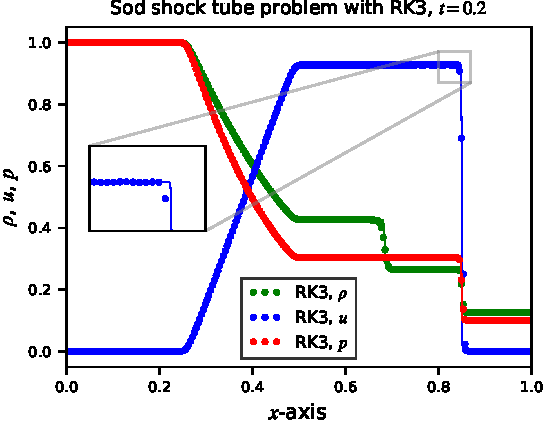
\includegraphics[width=\textwidth]{fig/sod_rk3}
        \caption{}\label{subfig:sod_rk3}
    \end{subfigure}
    \begin{subfigure}{0.49\textwidth}
        \centering
        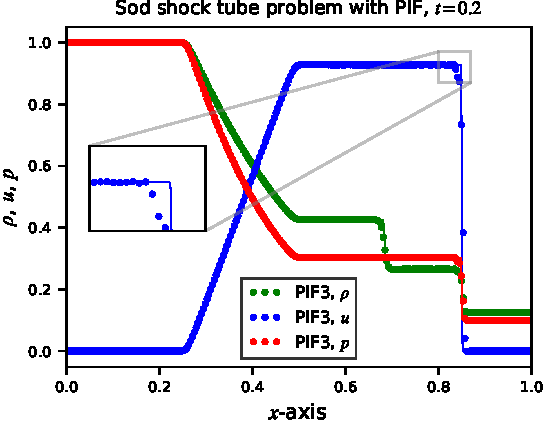
\includegraphics[width=\textwidth]{fig/sod_pif3}
        \caption{}\label{subfig:sod_pif3}
    \end{subfigure}
    \begin{subfigure}{0.49\textwidth}
        \centering
        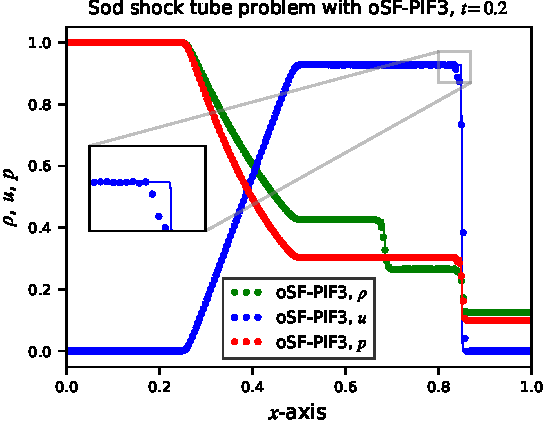
\includegraphics[width=\textwidth]{fig/sod_osf3}
        \caption{}\label{subfig:sod_osf3}
    \end{subfigure}
    \begin{subfigure}{0.49\textwidth}
        \centering
        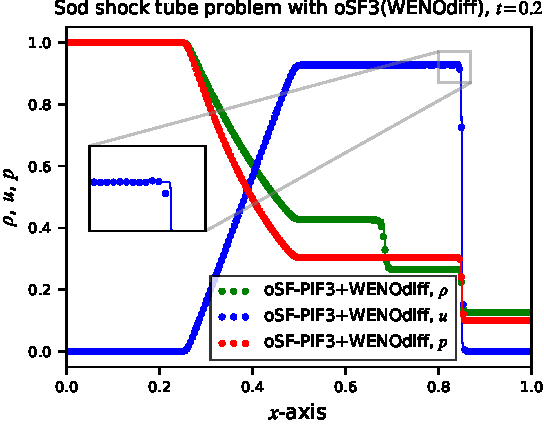
\includegraphics[width=\textwidth]{fig/sod_osf3_wenodiff}
        \caption{}\label{subfig:sod_osf3_wenodiff}
    \end{subfigure}
    \caption{Sod's shock tube problem at \( t = 0.2 \).
        The reference solutions are over-plotted
        as solid lines in each panel, which are resolved on a grid resolution of \( N_{x} = 1024 \)
        with RK3. The symbols in each panel represent the solution resolved on
        \( N_{x} = 256 \) grid cells with
        (\protect\subref{subfig:sod_rk3}) RK3,
        (\protect\subref{subfig:sod_pif3}) PIF3, and (\protect\subref{subfig:sod_osf3}) oSF-PIF3\@.
        (\protect\subref{subfig:sod_osf3_wenodiff}), the solution is resolved
        with oSF-PIF3 method combining with a new WENO-\textit{like} numerical differentiate operator,
        described as in~\crefrange{eq:pif_wenodiff_subs}{eq:pif_wenodiff_linear_weights}.
    }\label{fig:sod_third}
\end{figure}

The numerical solutions with the grid size of \( N_{x} = 256 \) at \( t = 0.2 \) are plotted
as symbols in each panel of~\cref{fig:sod_third}.
The solid lines on each panel represent the reference solution resolved on a more finer grid size,
\( N_{x} = 1024 \), by using WENO5+RK3.
The results resolved with recursive SF-PIF3 methods are omitted in this figure,
since the differences between SF-PIF3 and oSF-PIF3 are indistinguishable.

As illustrated in~\cref{subfig:sod_pif3} and~\cref{subfig:sod_osf3},
oSF-PIF3 method produce almost identical results of PIF3,
agreeing with the reference solutions and RK3's solutions in~\cref{subfig:sod_rk3}.
However, both in PIF3 and oSF-PIF3 methods,
there is a slight oscillation in the x-velocity immediately behind the shock front.
This small oscillation is originated from the use of
the conventional central differencing formulae in~\cref{eq:pif_central_dfdx}
for both oSF-PIF3 and PIF3.

The WENO-\textit{like} differencing strategy in~\crefrange{eq:pif_wenodiff_subs}{eq:pif_wenodiff_linear_weights}
can resolve this oscillation. As displayed in~\cref{subfig:sod_osf3_wenodiff},
the interchanging central differencing to WENO-differencing helps
to improve the performance of oSF-PIF3 at the shock,
suppressing the post-shock oscillations observed in~\cref{subfig:sod_pif3} and~\cref{subfig:sod_osf3}.
With this small fix, the oSF-PIF3 results are almost identical to the RK3 results in~\cref{subfig:sod_rk3}.
Computationally, the WENO-\textit{like} differencing adds extra floating-point operations,
which consequently slows down oSF-PIF's and SF-PIF's overall performance.
For this reason, the WENO-\textit{like} discretization was employed only
on the Sod's shock-tube test as a guide,
while it was opt-out on the rest of the test problems in this dissertation
where any unphysical has not been observed shock/discontinuity oscillations.


\subsection{Implosion test}\label{subsec:implosion}

The next problem to consider is the implosion test problem
introduced by Hui et al.~\cite{hui1999unified}.
An unsteady flow configuration is given as an initial condition which launches
a converging shock wave towards the domain center.
Following a more straightforward version by Liska and Wendroff~\cite{liska2003comparison},
the only right upper quadrant
of the original setup in~\cite{hui1999unified} is taken
as the simulation domain.
In this setup, the simulation is initialized on a region of a 2D square box,
\( \left[ 0, 0.3 \right] \times \left[ 0, 0.3 \right] \),
enclosed with reflecting walls,
in which case a converging shock wave is launched toward the lower-left corner
at $(x,y)=(0,0)$.
The initial shock wave bounces at the reflecting walls and produces a double Mach
reflection along two edges of $x=0$ and $y=0$.
Consequently, two jets are formed along the edges, moving toward the origin $(x,y)=(0,0)$ and collide
with each other. This two-jet collision then ejects a newly-formed jet into the diagonal direction
$x=y$. Reflecting shocks continuously interact with the diagonal jet, turning it into
a long and narrow shape over time. The observed structures of filaments and fingers
along with the diagonal jet and at its base are progressively intensified by the
Ritchmyer-Meshkov instability, a level of which depends sensitively on
numerical dissipation.

The shape of the jet is the key view point of
the implosion test since it is a good indicator of
a numerical method's symmetric property and numerical dissipation.
If the numerical scheme fails to maintain a high level of symmetry,
the jet will eventually be derailed off-diagonally and deformed over time.
Besides, an excess amount of numerical dissipation will
turn the jet into a less narrow and less elongated shape along the diagonal.

\begin{figure}
    \centering
    \begin{subfigure}{70mm}
        \centering
        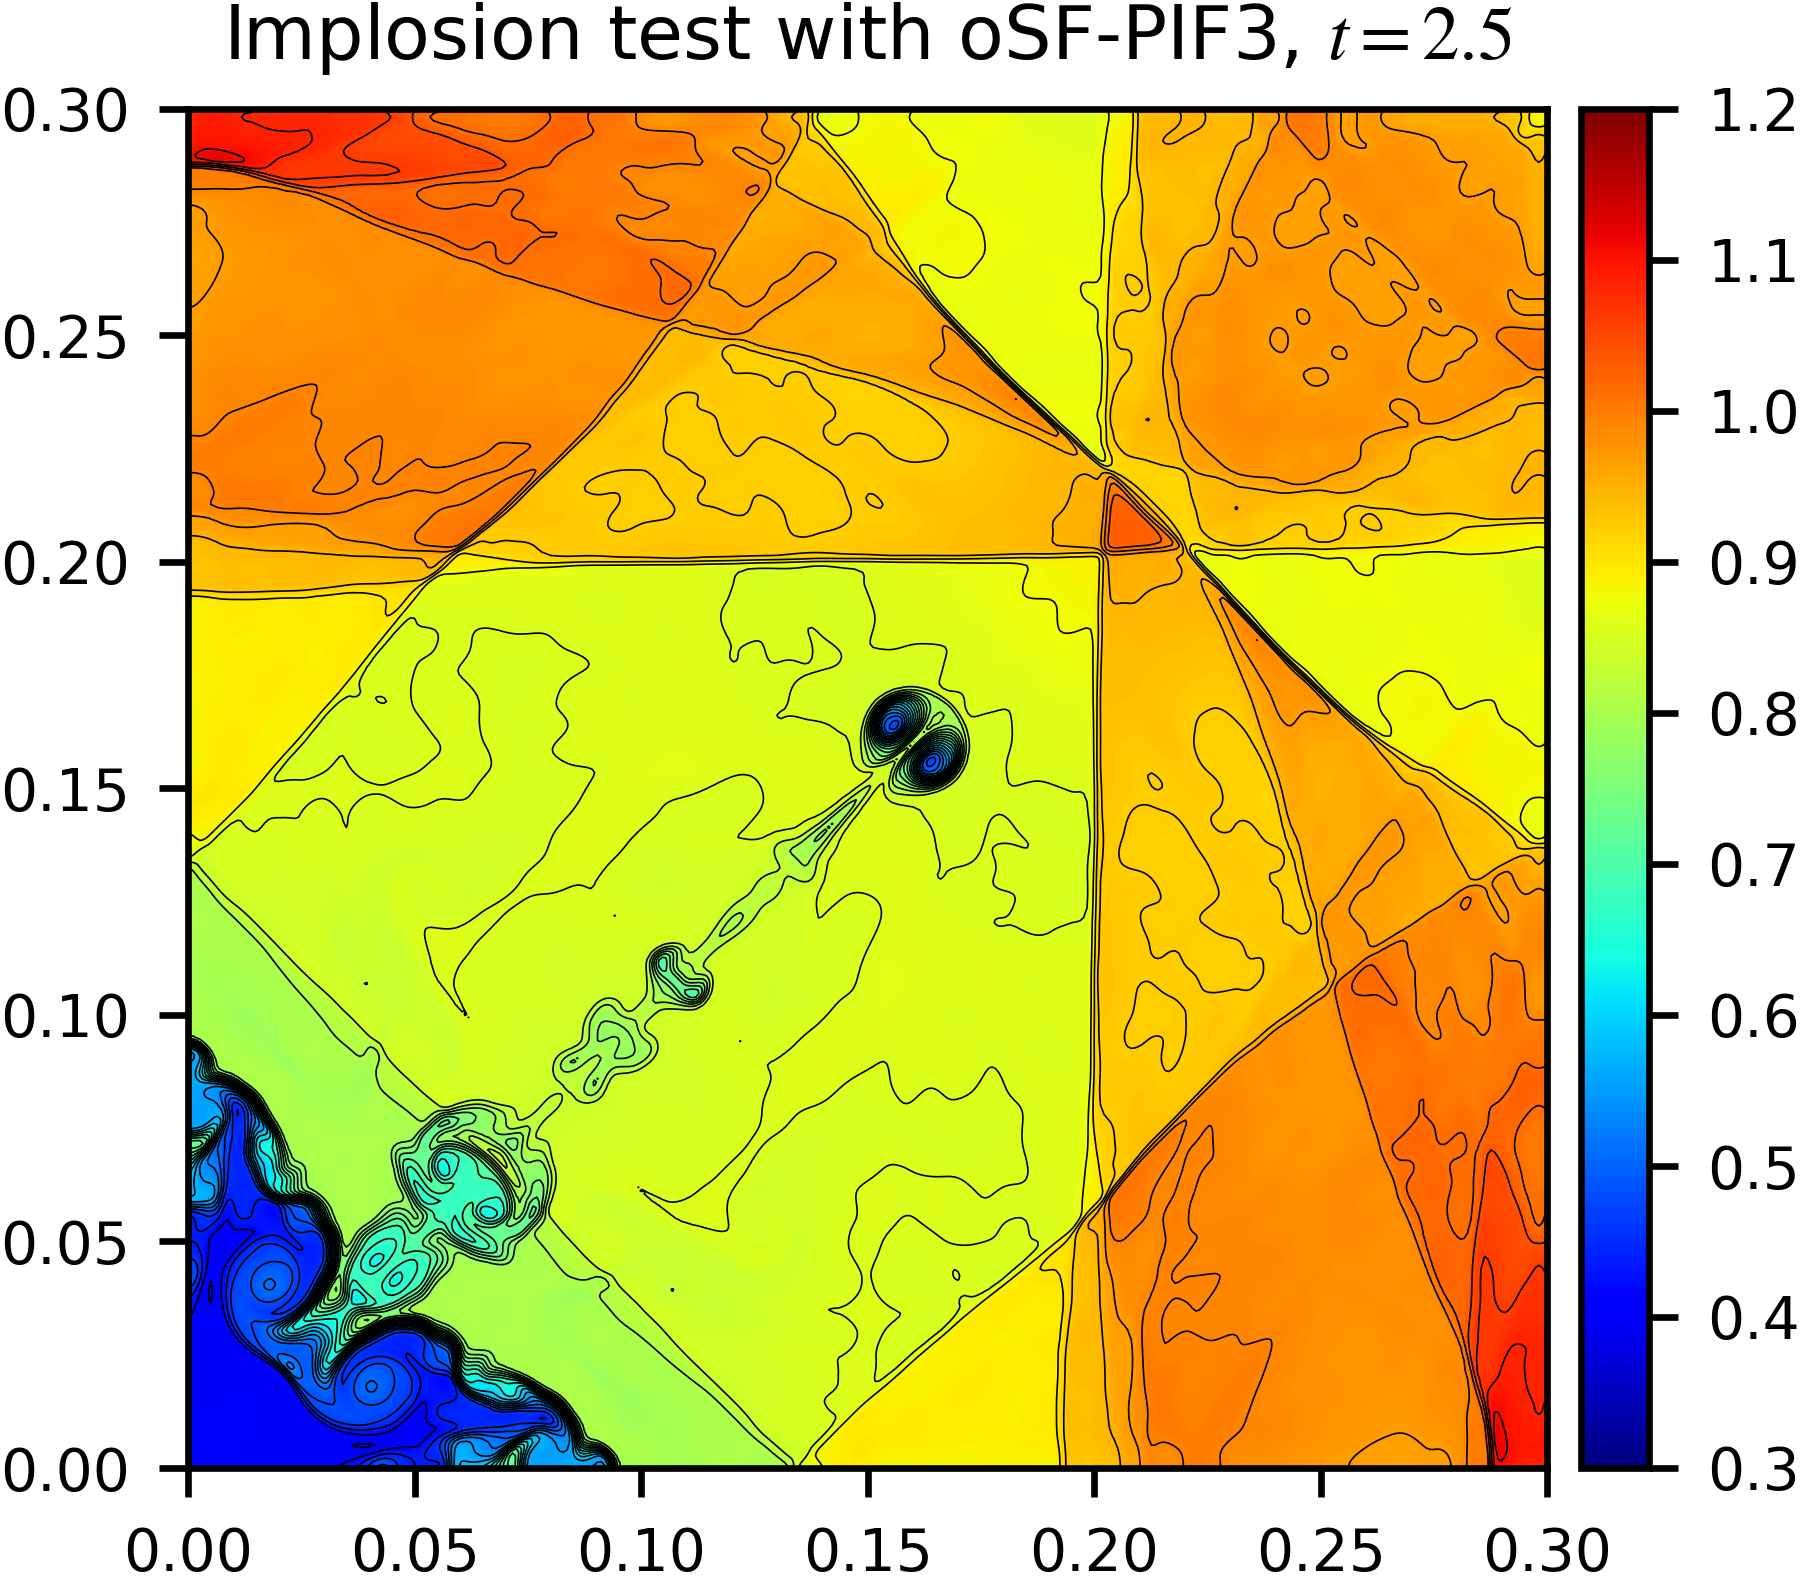
\includegraphics[width=0.95\textwidth]{fig/implosion_osf3.png}
    \end{subfigure}
    \begin{subfigure}{70mm}
        \centering
        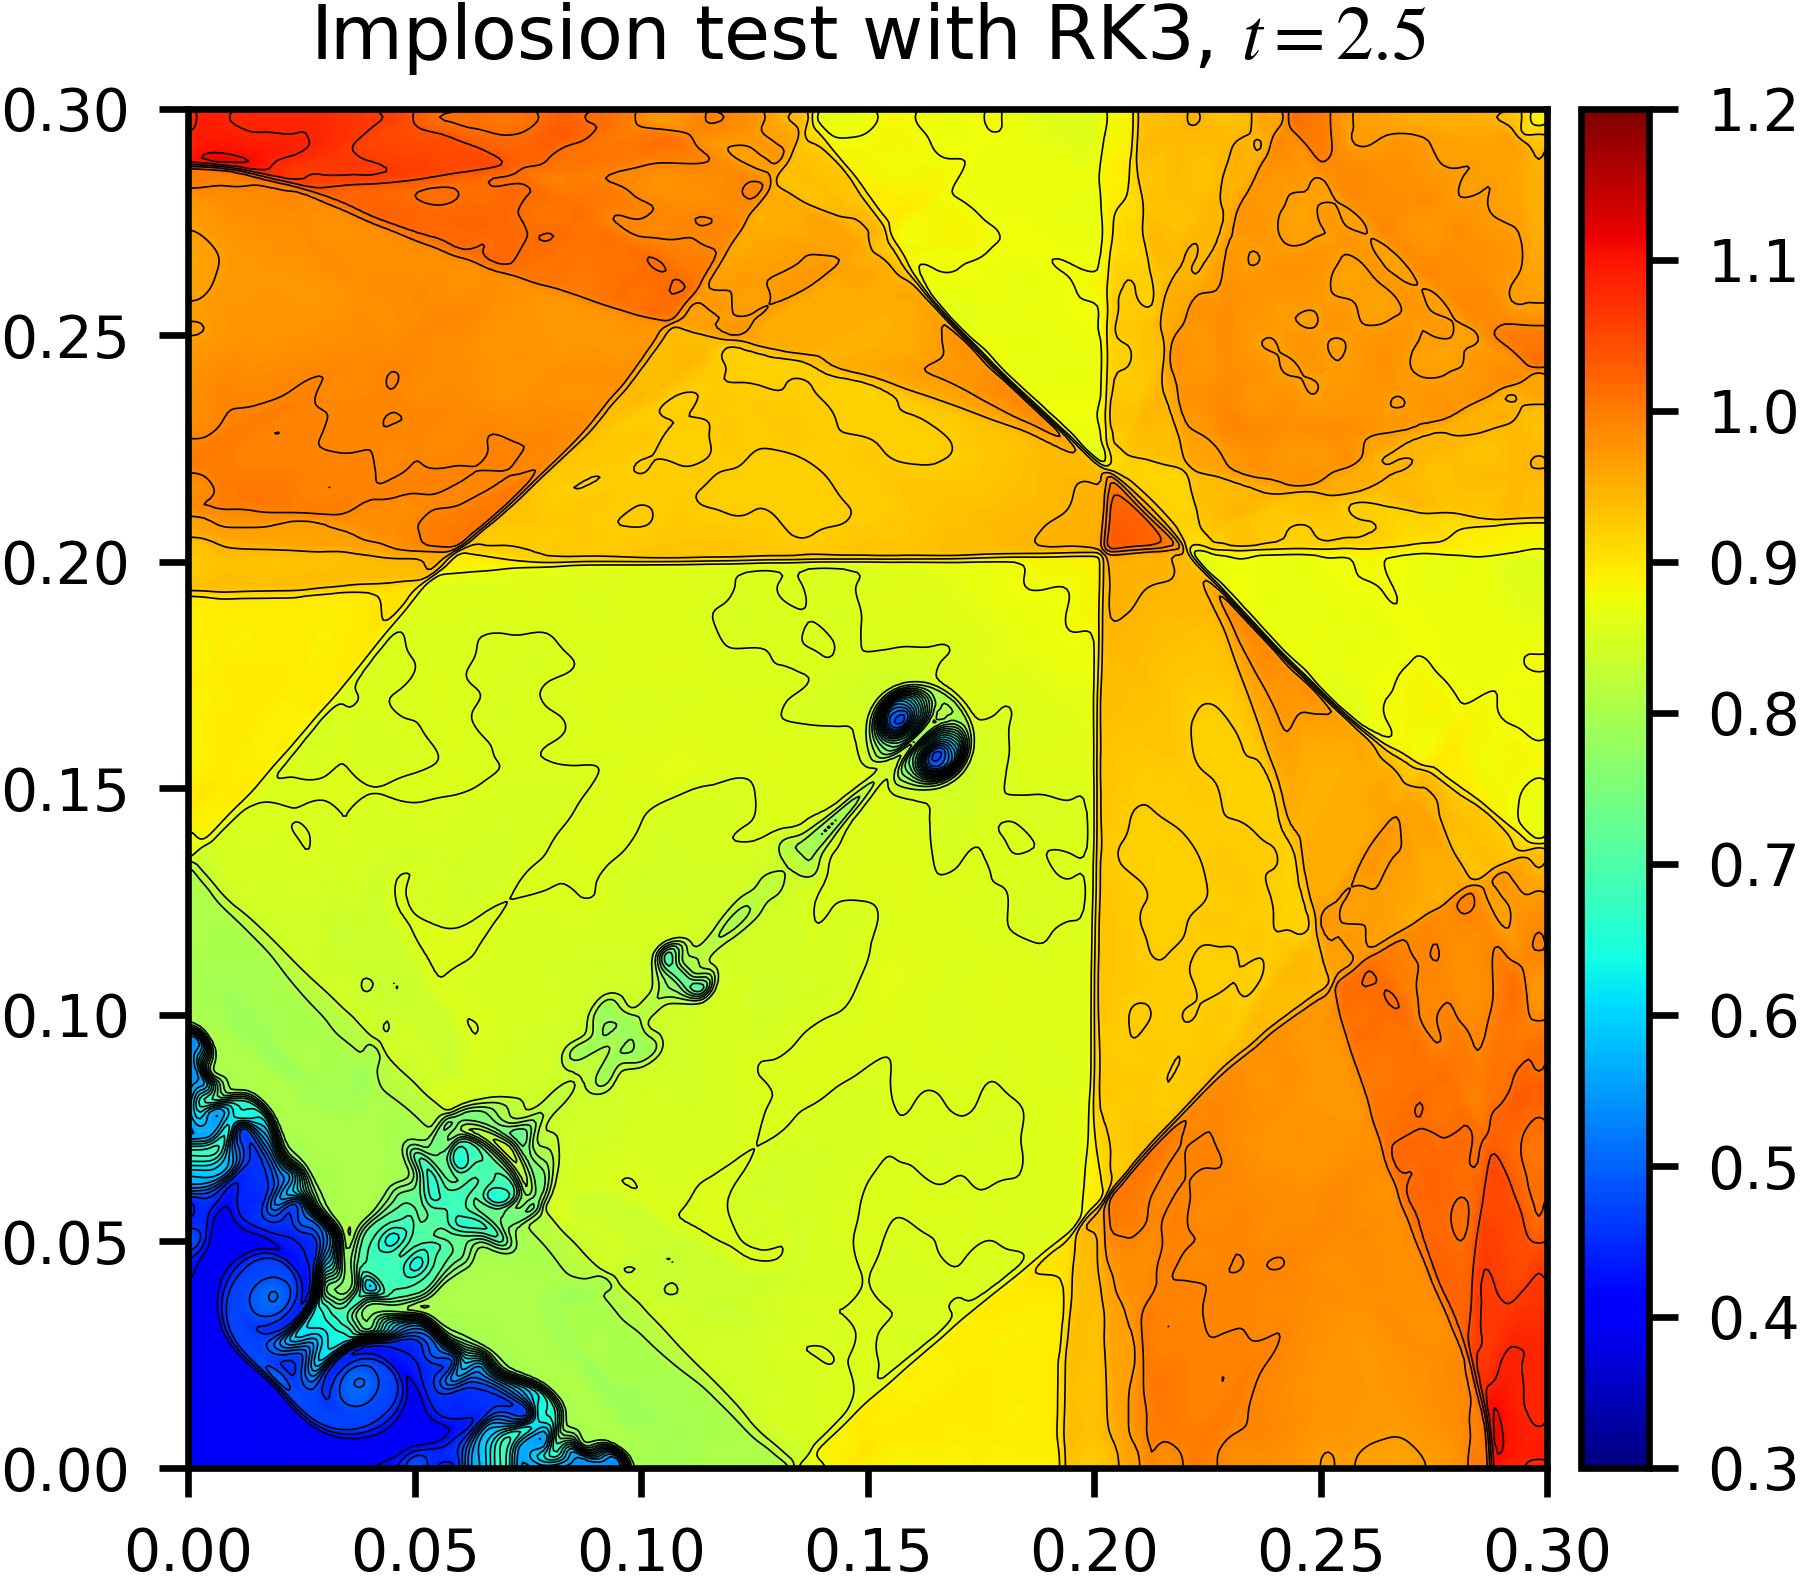
\includegraphics[width=0.95\textwidth]{fig/implosion_rk3.png}
    \end{subfigure}
    \caption{The density profile of the implosion test
        with oSF-PIF3 (left) and with RK3 (right).
        The color map ranges from \( 0.3 \) to \( 1.2 \), and
        40 evenly-spaced contour lines are over-plotted with
        the same range.
    }\label{fig:implosion}
\end{figure}

The density maps of the implosion test performed on
\( 400 \times 400 \) grid resolution at \( t = 2.5 \) are displayed in~\cref{fig:implosion}.
The result with oSF-PIF3 is on the left panel in \cref{fig:implosion} and RK3 on the right.
These results can also be directly compared with
Fig.~4.7 in~\cite{liska2003comparison} and Fig.~17 in~\cite{stone2008athena}.
The results of oSF-PIF3 (as well as RK3) present
the well-maintained symmetric jet along the diagonal direction
at a sufficient level.
At the same time, the shape of the diagonal jet using oSF-PIF3 matches
well with the shape using RK3,
and hence is sufficient to demonstrate that the numerical dissipation in oSF-PIF3
is well-managed compared with RK3.


\subsection{Shallow water equations}\label{subsec:shallow}



\section{SF-PIF method with WENO-JS}\label{sec:result_wenojs}

\noter{All recursive SF-PIFs}

\subsection{The Shu-Osher problem (rotated \(\ang{45}\))}\label{subsec:shu45_weno}

\subsection{2D Riemann problem: Configuration 3}\label{subsec:2drp_c3_weno}

\subsection{Double Mach reflection}\label{subsec:dmr_weno}



\section{SF-PIF method with GP-WENO}\label{sec:result_gpweno}

\subsection{Hyperparameters}\label{subsec:hyper_params_gpweno}

\subsection{2D Riemann problem: Configuration 3}\label{subsec:2drp_c3_gp}

\noter{what else...}

